% -*- TeX-master: "main"; fill-column: 72 -*-

\section{Proposed syntax and semantics}
\label{syntax}

In this section, we define the syntax and semantics of the Flux Balance
Constraints package for SBML Level~3 Version~1.  We expound on the various
data types and constructs defined in this package, then in \sect{examples},
we provide complete examples of using the constructs in example SBML
models.

% -----------------------------------------------------------------------------
\subsection{Namespace URI and other declarations necessary for using this package}
\label{xml-namespace}

Every SBML Level~3 package is identified uniquely by an XML namespace URI.
For an SBML document to be able to use a given SBML Level~3 package, it
must declare the use of that package by referencing its URI.  The following
is the namespace URI for this version of the Flux Balance Constraints
package for SBML Level~3 Version~1:
\begin{center}
\uri{http://www.sbml.org/sbml/level3/version1/fbc/version1}
\end{center}

In addition, SBML documents using a given package must indicate whether
understanding the package is required for complete mathematical
interpretation of a model, or whether the package is optional.  This is
done using the attribute \token{required} on the \token{<sbml>} element in
the SBML document.  For the Flux Balance Constraints package, the value of
this attribute must be set to \val{true}.

The following fragment illustrates the beginning of a typical SBML model
using SBML Level~3 Version~1 and this version of the Flux Balance
Constraints package:

\begin{example}
<?xml version="1.0" encoding="UTF-8"?>
<sbml xmlns="http://www.sbml.org/sbml/level3/version1/core" level="3" version="1"
      xmlns:fbc="http://www.sbml.org/sbml/level3/version1/fbc/version1" fbc:required="true">
\end{example}

\begin{figure}[h]
  \centering
  % Requires \usepackage{graphicx}
  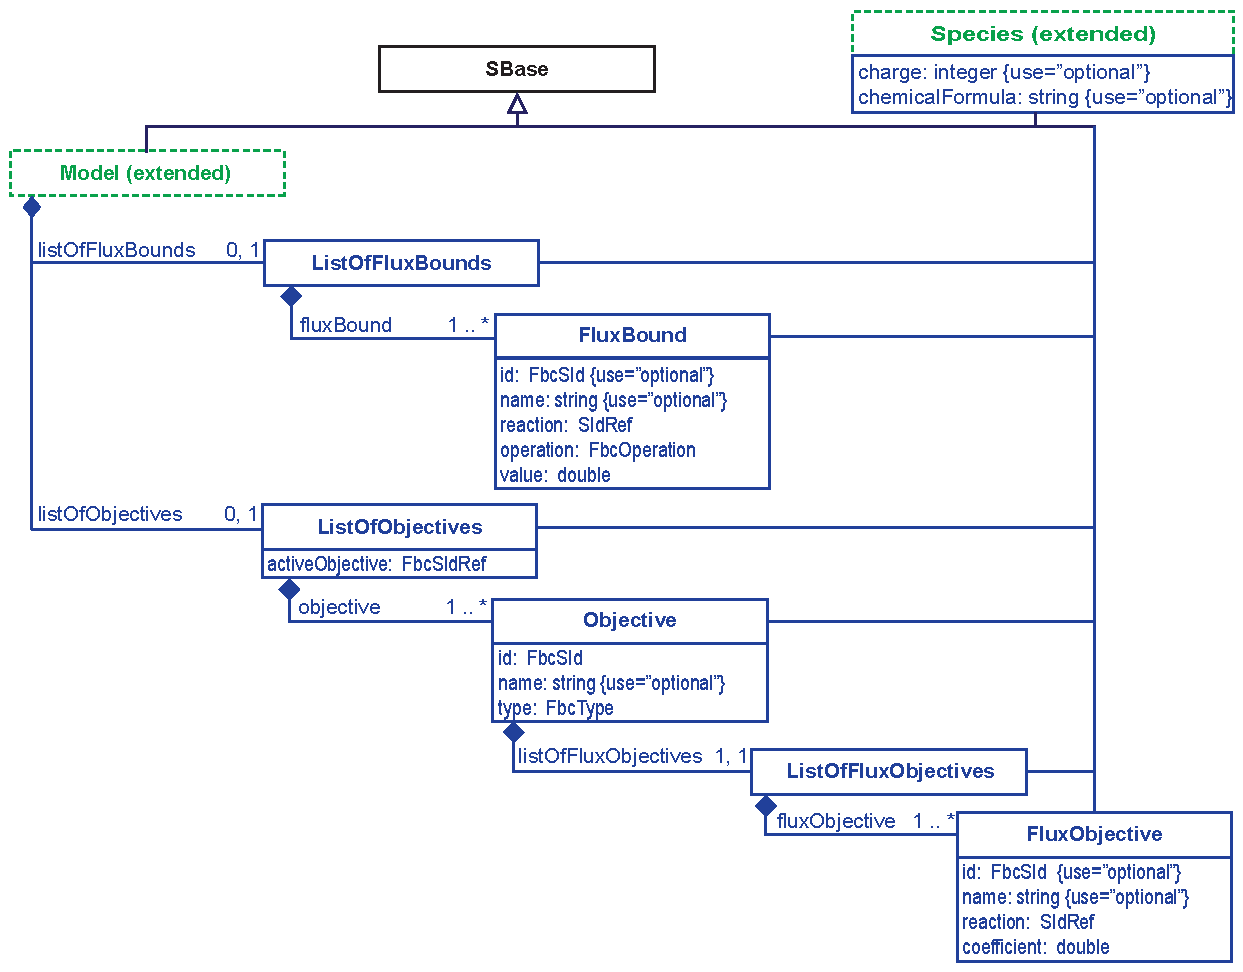
\includegraphics[width=\textwidth]{images/fbc_uml.pdf}\\
  \caption{A UML representation of the Flux Balance Constraints package classes. See \ref{conventions}} for conventions related to this figure. \label{fig:fbc_uml}
\end{figure}

\subsection{Primitive data types}
Section~3.1 of the \sbmlthreecore specification defines a number of
primitive data types and also uses a number of XML Schema 1.0 data
types~\citep{biron:2000}.  More specifically we make use of \primtype{integer}, \primtype{double}, \primtype{string}, \primtype{SIdRef} and \primtype{enum}. In addition we make use of two new primitives \primtype{FbcSId} and \primtype{FbcSIdRef}, see \ref{fig:fbc_uml} for the interrelation between these entities.

\subsubsection{Type \primtypeNC{FbcSId}}
\label{primtype-fbcsid}

The type \primtype{FbcSId} is derived from \primtype{SId} (\sbmlthreecore specification Section~3.1.7) and has identical syntax. The \primtype{FbcSId} type is used as the data type for the identifiers of \FluxBound (\ref{fluxbound-class}) and \Objective (\ref{objective-class}) classes. By using a separate identifier type we differentiate them from others defined in the \SBML model and thus ensuring data encapsulation. In addition the \Objective class \primtype{FbcSId} provides an identifier to the \Objective which is set as active. The equality of \primtype{FbcSId} values is determined by an exact character sequence match and therefore comparisons of these identifiers must be performed in a case-sensitive manner.

\subsubsection{Type \primtypeNC{FbcSIdRef}}
\label{primtype-fbcsidref}

Type \primtype{FbcSIdRef} is used for all attributes that refer to
identifiers of type \primtype{FbcSId}.  Derived from
\primtype{FbcSId} it has the restriction that the value of an
attribute having type \primtype{FbcSIdRef} must match the value of a
\primtype{FbcSId} attribute in the current model. In the FBC package the \ListOfObjectives has an attribute of this type that is used to refer to an `active' \Objective.

\subsection{The extended \class{Model} class}
\label{sbml-model}
\label{listoffluxbounds-class}
\label{listofobjectives-class}

The \SBML \Model class is extended with the addition of two children, i.e. a \token{listOfFluxBounds} and a \token{listOfObjectives}.


\subsubsection{The lists of objectives and flux bounds}
As shown in \ref{fig:fbc_uml} the \ListOfFluxBounds and \ListOfObjectives are derived from \SBase and inherit \token{metaid} and \token{sboTerm}, as well as the subcomponents for \Annotation and \Notes. Both of these list are required to contain one or more elements when defined, however, the lists themselves are optional. Unlike most other \SBML \textsf{\textbf{ListOf\rule{0.15in}{0.5pt}}} classes, \ListOfObjectives introduces an additional required attribute \token{activeObjective}.

\paragraph{The \token{activeObjective} attribute}
\label{activeObjective-attribute}
This attribute contains a \val{value} of type \primtype{FbcSIdRef} that can only refer to an existing \Objective \primtype(FbcSId). This required attribute exists so that when multiple \Objective's are included in a single model, the model will always be well described i.e. there is a single, primary objective function which closes the solution space.

\subsection{The extended \class{Species} class}
\label{sbml-species}
\label{species-class}

The \FBC package extends the \SBML \Species class with the addition of two attributes:
\begin{itemize}
  \item an optional attribute \token{charge} which contains an \primtype{integer} referring to the \Species objects charge (as defined in \SBML Level 2)
  \item an optional attribute \token{chemicalFormula} containing a \primtype{string} that represents the \Species objects elemental composition.
\end{itemize}

\paragraph{The \token{chemicalFormula} attribute}
\label{chemicalFormula-attribute}
While there are many ways of referring to an elemental composition the purpose of the \token{chemicalFormula} attribute is to allow reaction balancing and validation which is particularly important in constraint based models. To this end it is recommended that the format of \token{chemicalFormula} should follow the Hill system (or notation). Here the number of carbon atoms in a molecule is indicated first, followed by the number of hydrogen atoms and then the number of all other chemical elements in alphabetical order. When the formula contains no carbon; all elements, including hydrogen, are listed alphabetically \cite{hillsystem, hillwikipedia}.

\subsection{The \FBC \class{FluxBound} class}
\label{fluxbound-class}

\FluxBound is a new \FBC class derived from \SBML \SBase that inherits \token{metaid} and \token{sboTerm}, as well as the subcomponents for \Annotation and \Notes. The purpose of this class is to hold a single (in)equality that provides the maximum or minimum value that a reaction flux can obtain at steady state. It is is relatively straight forward and implements four attributes.

\begin{itemize}
  \item An \token{id} attribute that contains an \primtype{FbcSId},
  \item a \token{reaction} attribute that takes an \primtype{SIdRef} and can take \SBML \Reaction \primtype{SId} as a value,
  \item an \token{operation} attribute of type \primtype{enum} that can take a limited set of boolean operators (see text for details),
  \item \token{value} an attribute that takes a \primtype{double} value representing the bound. This may include $\pm\infty$ encoded as the value \val{INF}
\end{itemize}

\paragraph{The \token{operation} attribute}
The \token{operation} attribute represents a mathematical (in)equality of the form <\token{reaction}> <\token{operator}> <\token{value}> e.g.
 \begin{quote}\center
 R$_{5}$ >= 0\newline
 R$_{5}$ <~ $\infty$\newline
 R$_{7}$ = 1.0\newline
\end{quote}
An enumerated type that can take one of the following values:
\begin{eqnarray*}
% I'm using \mapsto until I can find the proper symbol - bgoli
\label{fb-operation-enum}
 \nonumber
  <= & \mapsto & \val{lessEqual}\\
  >= & \mapsto & \val{greaterEqual}\\
  < & \mapsto & \val{less}\\
  > & \mapsto & \val{greater}\\
  = & \mapsto & \val{equal}\\
  \textrm{undefined} & \mapsto & \val{unknown}
\end{eqnarray*}
%\begin{itemize}
%  \item \val{lessEqual}, equivalent to $<=$
%  \item \val{greaterEqual}, equivalent to $>=$
%  \item \val{less}, equivalent to $<$
%  \item \val{greater}, equivalent to $>$
%  \item \val{equal}, equivalent to $=$
%  \item \val{unknown} representing an undefined operator
%\end{itemize}


\subsection{The \FBC \class{Objective} class}
\label{objective-class}
\label{listoffluxobjectives-class}

As shown in \ref{fig:fbc_uml} the \FBC \Objective class is derived from \SBML \SBase and inherits \token{metaid} and \token{sboTerm}, as well as the subcomponents for \Annotation and \Notes. An integral component in a complete description of a steady-state model is the so-called `objective function' which generally consist of a linear combination of model variables (fluxes) and a sense (direction). In the \FBC package this concept is succinctly captured in the \Objective class containing three required attributes:
\begin{itemize}
  \item \token{id} an attribute that can only contain an \primtype{FbcSId},
  \item \token{type} an \primtype{enum} (see below),
  \item \token{listOfFluxes} which contains a \ListOfFluxObjectives.
\end{itemize}

\paragraph{The \token{type} attribute}
The \token{type} attribute contains an \primtype{enum} which represents the sense of the optimality constraint and can take one of three values:
\begin{eqnarray*}
% I'm using \mapsto until I can find the proper symbol - bgoli
\label{obj-type-enum}
 \nonumber
  maximize & \mapsto & \val{maximize}\\
  minimize & \mapsto & \val{minimize}\\
 \textrm{undefined} & \mapsto & \val{unknown}
\end{eqnarray*}

\paragraph{The \token{listOfFluxes} attribute}
The \ListOfFluxObjectives is derived from and functions like a typical \SBML \textsf{\textbf{ListOf\rule{0.15in}{0.5pt}}} class with the proviso that it cannot be empty and must contain one or more \token{fluxObjective} attributes of type \FluxObjective (see \ref{fluxobjective-class}).

\subsection{The \FBC \class{FluxObjective} class}
\label{fluxobjective-class}

As shown in \ref{fig:fbc_uml} the \FBC \FluxObjective class is derived from \SBML \SBase and inherits \token{metaid} and \token{sboTerm}, as well as the subcomponents for \Annotation and \Notes.

The \FluxObjective class is a relatively simple container for a model variable weighted by a signed linear coefficient:
\begin{itemize}
  \item \token{id} an attribute that contains an \primtype{SId} that is restricted to refer only to an \SBML \Reaction,
  \item \token{coefficient} a \primtype{double}.
\end{itemize}
